\chapter{Visão Geral dos Resultados}
Os achados corroboram amplamente a presença de vieses cognitivos sistemáticos nas percepções econômicas do eleitorado brasileiro e evidenciam um papel preponderante da orientação ideológica em comparação ao mero nível de informação. Para visualizar o padrão Geral–Esclarecido–Economistas, ver \autoref{fig:deficit}, \autoref{fig:ajuda} e \autoref{fig:impostos}. As figuras desta seção derivam dos modelos logit definidos na Seção 3.4 e do contrafactual de “público esclarecido” apresentado na Seção 3.5. Note que o contrafactual é estimado apenas para o perfil “público esclarecido”; as barras de Público e Economistas correspondem às médias observadas de cada grupo.

Nas figuras, o eixo horizontal apresenta as médias na escala 0–2 e o eixo vertical exibe três perfis: Público ($\textit{econ}=0$), Público esclarecido (contrafactual) e Economistas ($\textit{econ}=1$). Essas médias combinam valores observados (Público e Economistas) e predições do contrafactual que simula como os economistas responderiam caso não tivessem formação específica ($\textit{econ}=0$), mantendo as demais covariáveis constantes; são predições no espaço da resposta, não coeficientes $\beta$ de uma variável indicadora. A leitura é direta: compara-se o comprimento das barras — quando o grupo “esclarecido” se aproxima dos economistas, isso indica efeito informacional da formação em Economia; quando se confunde com o público, não há efeito de formação (prevalecem ideologia e valores); quando fica entre ambos, o efeito é parcial.


\begin{figure}[htbp]
\centering
\caption{Médias de concordância com a afirmação ``O déficit federal é grande demais'' para o público geral, o público ``esclarecido'' e os economistas.}
\includegraphics[width=0.8\textwidth]{Textuais/analise/imagens/déficit_federal_grande.png}
\notafig
\label{fig:deficit}
\end{figure}

\begin{figure}[htbp]
\centering
\caption{Médias de concordância com a afirmação ``O gasto com ajuda externa é alto demais'' para o público geral, o público ``esclarecido'' e os economistas.}
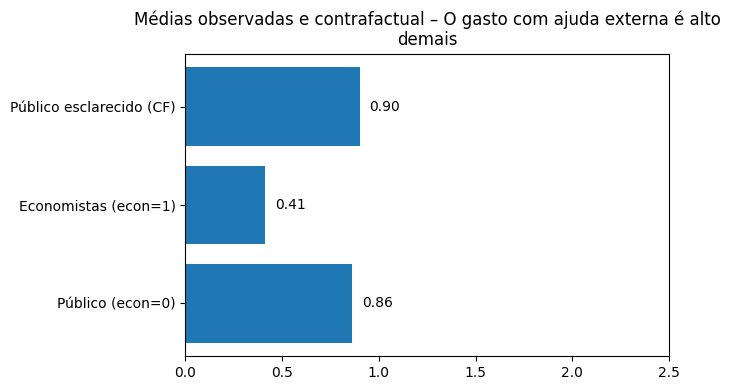
\includegraphics[width=0.8\textwidth]{Textuais/analise/imagens/gasto_ajuda_externa.png}
\notafig
\label{fig:ajuda}
\end{figure}

\begin{figure}[htbp]
\centering
\caption{Médias de concordância com a afirmação ``Os impostos são muito altos'' para o público geral, o público ``esclarecido'' e os economistas.}
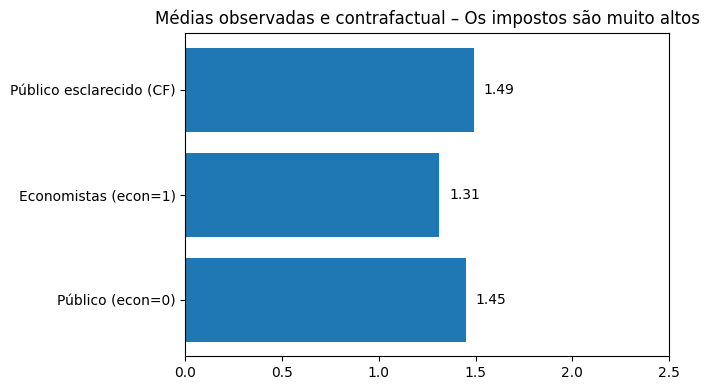
\includegraphics[width=0.8\textwidth]{Textuais/analise/imagens/impostos_muito_altos.png}
\notafig
\label{fig:impostos}
\end{figure}

De forma resumida, a análise integrada dos modelos logit estimados permite destacar os seguintes pontos centrais (ver Tabela~\ref{tab:achados}): 

\begin{enumerate}[label=\alph*)]

    \item \textbf{Vieses generalizados}: na \textit{maioria} das 57 questões analisadas, identificam-se diferenças sistemáticas entre grupos de respondentes, compatíveis com vieses descritos na literatura (antimercado, antiestrangeiro, antitrabalho, pessimista) \cite{The_Myth_of_the_Rational_Voter}.

    \item \textbf{Influência dominante da ideologia}: em grande parte das variáveis dependentes (DVs), o coeficiente associado ao espectro ideológico foi estatisticamente significativo (com frequência \(p<0{,}01\)), ao passo que o coeficiente de formação em Economia (indicador de conhecimento especializado) alcançou significância em um subconjunto menor de DVs. Ademais, a magnitude típica dos efeitos ideológicos superou a dos efeitos de conhecimento: na \textit{escala de log-odds} dos modelos ordenados, \(|\beta_{\text{ideologia}}|\) concentrou-se tipicamente entre 0{,}5 e 0{,}9, enquanto \(|\beta_{\text{econ}}|\) se situou em torno de 0{,}2–0{,}7 nos casos significativos. Em termos substantivos, posicionar-se à direita (versus à esquerda) alterou substancialmente as probabilidades de concordar com proposições como “a dívida pública é grande demais” (ver \autoref{fig:deficit}) ou “as políticas de cotas são excessivas”, ao passo que possuir formação em Economia (versus ser leigo) produziu efeito menor, embora não desprezível.
    
    \item \textbf{Consensos técnicos versus divisões valorativas}: alguns itens revelam consenso amplo entre público e economistas (ausência de viés), sobretudo em princípios econômicos tradicionais; já em temas socioeconômicos carregados de valores, observam-se clivagens acentuadas por ideologia, independentemente de conhecimento.
    
    \item \textbf{Conhecimento como “freio” pontual}: a formação econômica mostrou impacto notável em corrigir percepções factuais equivocadas em certos itens — isto é, quando a desinformação objetiva era o motor dominante — aproximando as respostas de economistas e de leigos “esclarecidos”, ainda que sem alterar preferências guiadas por valores.
    
    \item \textbf{Robustez dos padrões}: os resultados mantêm-se consistentes com a inclusão de controles demográficos e socioeconômicos, sugerindo que os efeitos de ideologia e conhecimento não decorrem de fatores de confusão evidentes.
\end{enumerate}

\subsection{O público “esclarecido” como régua entre ideologia e informação} 

Para quantificar separadamente os efeitos da ideologia e do conhecimento, definiu-se o chamado \textit{público esclarecido} como um experimento contrafactual: trata-se da opinião média prevista caso os respondentes leigos tivessem nível de informação equivalente ao dos economistas, mantendo-se seus demais atributos constantes (em particular, conserva-se a distribuição original de orientações ideológicas). Em outras palavras, o público esclarecido simula qual seria a percepção popular na ausência de déficits de conhecimento técnico. Como era de se esperar, nas figuras observamos que esse grupo hipotético tende a ocupar uma posição intermediária entre o público geral e os economistas. 

Essa posição serve como uma régua de comparação que permite discernir, em cada questão, o peso relativo da ideologia (diferença entre as opiniões do público esclarecido e dos economistas) em contraste com o peso da informação (diferença entre o público geral e o esclarecido). Se a introdução de conhecimento técnico (passando do público geral ao esclarecido) pouco altera a opinião média, conclui-se que o fator ideológico domina naquela questão; por outro lado, se o público esclarecido praticamente converge com os economistas, infere-se que o gap original decorria majoritariamente de desinformação. 

A seguir, organizam-se os achados por blocos temáticos, discute-se o peso relativo de ideologia e informação e, por fim, avaliam-se robustez, limitações e implicações à luz das hipóteses do estudo.

\begin{quadro}[!htb]\centering\footnotesize
\caption{Principais achados dos resultados empíricos}\label{tab:achados}
\begin{tabular}{p{5.5cm} p{9.5cm}}
\toprule
\textbf{Achado-chave} & \textbf{Evidências selecionadas} \\
\midrule
\textbf{Ideologia como filtro dominante} & Coeficientes ideológicos significativos na \textit{maioria} das 37 regressões (em muitos casos com \(p<0{,}01\)). Efeito típico: \(|\beta_{\text{ideologia}}|\approx0{,}5\text{–}0{,}9\) (log-odds), superando o impacto do conhecimento. Ex.: respondentes à direita tenderam mais a ver a dívida pública como “grande demais” e a rejeitar maior intervenção estatal; à esquerda verificou-se o padrão inverso. \\
\textbf{Conhecimento técnico corrige desinformação} & Coeficientes de “formação em Economia” significativos em cerca de um terço dos modelos, geralmente \(|\beta_{\text{econ}}|\approx0{,}2\text{–}0{,}7\). Ex.: economistas (controlada a ideologia) discordaram em proporção maior de “gasta-se muito com ajuda externa” (\autoref{fig:ajuda}), ajustando uma crença popular que superestima essa rubrica; de modo análogo, mostraram menor alarme em relação ao déficit público (\autoref{fig:deficit}), em linha com critérios técnicos de sustentabilidade fiscal \cite{The_Myth_of_the_Rational_Voter}. \\
\textbf{Consenso em bases econômicas} & Diversas questões de economia básica e reformas estruturais apresentaram concordância ampla entre grupos. Ex.: “A reforma tributária é necessária” obteve concordância elevada entre leigos e economistas (médias de resposta \(\approx1{,}81\) e \(\approx1{,}94\), respectivamente), sem clivagem ideológica robusta. Em contrapartida, \textit{reforma previdenciária} e \textit{trabalhista} exibem apoio majoritário, porém com gradiente ideológico significativo (direita apoia mais). \\
\textbf{Clivagens socioideológicas acentuadas} & Em itens distributivos e de avaliação do setor privado — p.ex., “empresas lucram demais”, “salários de altos executivos são excessivos”, “ações afirmativas dão vantagens demais” — observa-se clivagem marcada: o público leigo mostrou-se relativamente mais crítico que economistas, e as respostas polarizaram por ideologia. A interpretação é compatível com o papel das narrativas político-emocionais na formação de crenças \cite{westen2007political}. \\
\textbf{Viés pessimista e outras tendências} & Identifica-se um viés pessimista relevante: parcela expressiva dos eleitores avaliou a situação (atual e futura) de forma mais negativa do que economistas, notadamente em desigualdade e renda real ao longo do tempo; padrões transversais por sexo e idade também emergem (homens mais céticos quanto à regulação e menos críticos a salários executivos; faixas de 46–55 e 66+ mais sensíveis a temas como juros e corrupção). \\
\bottomrule
\end{tabular}
\end{quadro}

\section{Resultados por Bloco Temático de Variáveis Dependentes}
Os padrões observados permitem agrupar as questões em blocos temáticos conforme suas dinâmicas substantivas comuns. Em vez de examinar cada pergunta isoladamente, a seguir sintetizamos os resultados por conjunto de itens relacionados, destacando exemplos representativos e conectando-os às hipóteses teóricas relevantes.

\subsection{Consenso em Políticas Econômicas Estruturais}
Em diversas perguntas sobre princípios de economia e reformas estruturais observou-se convergência ampla nas opiniões dos segmentos analisados. Em particular, no item ``\textit{A reforma tributária é necessária}'' verificou-se concordância praticamente unânime entre respondentes com e sem formação em Economia (médias de resposta, respectivamente, $\approx1{,}94$ e $\approx1{,}81$, em escala Likert de 0 sendo ``discordo totalmente'' a 2 sendo ``concordo totalmente''), sem diferenças ideológicas ou educacionais robustas. Por outro lado, em ``\textit{A reforma da previdência é necessária}'' e ``\textit{A reforma trabalhista é necessária}'', embora o apoio seja majoritário, persiste o gradiente ideológico estatisticamente significativo (maior apoio entre respondentes à direita). Em síntese, identifica-se um núcleo de consenso real em matérias estruturais (p.\,ex., a necessidade de revisar o arranjo tributário), ao passo que, em outras reformas, o apoio amplo convive com clivagens ideológicas previsíveis. Essa configuração é compatível com a distinção de \cite{sowell2007conflict} entre ``visões'' de mundo: quando o diagnóstico técnico é menos controverso moralmente, mesmo agentes com informação limitada tendem a alinhar suas crenças ao consenso pericial.

\subsection{Divergências Ideológicas em Questões Socioeconômicas}
Em contraste com os consensos acima, um segundo bloco reúne itens com conotação ideológica/distributiva mais saliente, em que despontam divergências marcantes entre grupos. Entram aqui enunciados como ``\textit{As empresas têm lucros demasiadamente altos}'', ``\textit{Os salários dos altos executivos são excessivos}'', ``\textit{As ações afirmativas dão vantagens demais para minorias}'', ``\textit{Ter mais mulheres na força de trabalho é algo positivo}'' e “\textit{os impostos são muito altos}”, que exibe gradiente ideológico nítido (\autoref{fig:impostos}). Os resultados indicam que o público leigo se mostrou relativamente mais crítico que os economistas em relação a lucro privado e remuneração executiva, com clivagem ideológica pronunciada (maior concordância à esquerda e menor à direita). 

Tal padrão é compatível com o viés antimercado discutido por \citeonline{The_Myth_of_the_Rational_Voter}, segundo o qual eleitores tendem a superestimar efeitos negativos atribuídos ao mercado e a favorecer correções estatais. A leitura também dialoga com a tipologia de visões proposta por \citeonline{sowell2007conflict}: a ``visão constrangida'' tende a reconhecer trade-offs e a valorizar mecanismos de mercado, ao passo que a ``visão não constrangida'' mostra maior propensão a soluções igualitaristas. Ademais, como argumenta \citeonline{westen2007political}, identidades e afetos partidários modulam a recepção de evidências, de modo que direita e esquerda filtram o mesmo fato por lentes normativas distintas. Em termos empíricos, a variável de \textit{espectro ideológico} emerge significativa na maioria desses itens polarizadores, configurando um espelhamento ideológico robusto: esquerda associa problemas a ``falhas de mercado'' e demanda regulação/redistribuição; direita associa problemas a ``falhas de governo'' e demanda restrição a gastos/intervenção.

\subsection{Questões de Viés Informacional e Correções pelo Conhecimento}
Um terceiro padrão envolve itens nos quais a assimetria informacional aparece como mecanismo central de divergência entre opinião popular e leitura técnica. Nesses casos, controlada a ideologia, a formação em Economia associa-se a respostas significativamente distintas do público leigo, sugerindo que a variação decorre de diferenças de informação.

O exemplo mais claro é ``\textit{O gasto com ajuda externa é alto demais}''. Aqui, identificou-se efeito ideológico positivo (respondentes mais à direita concordam mais) e um efeito corretivo de formação (coeficiente negativo significativo para a dummy de Economia): economistas, independentemente de sua orientação política, tendem a discordar do enunciado, coerentes com o fato de que tal rubrica representa parcela diminuta do orçamento. Em outras palavras, a informação especializada reduz uma percepção equivocada que atravessa o espectro político. Esse ajuste é visível no contraste entre as três barras de \autoref{fig:ajuda}.

Padrão análogo surge em ``\textit{O déficit federal é grande demais}'': o coeficiente ideológico é positivo e altamente significativo (maior preocupação à direita), enquanto a dummy de formação em Economia é negativa e significativa, indicando menor alarmismo entre os tecnicamente informados (médias $\approx1{,}51$ no público leigo versus $\approx1{,}12$ entre economistas). Essa combinação sustenta a afirmação anterior acerca de viés \textit{pessimista} do eleitor e de que o conhecimento atua como \textbf{freio epistêmico}, atenuando leituras alarmistas infundadas. O padrão de menor alarmismo técnico aparece em \autoref{fig:deficit}.

Há, ainda, casos em que o público tende a \textit{subestimar} problemas estruturais pouco salientes intuitivamente. Em ``\textit{A produtividade aumenta devagar demais}'' e em ``\textit{Empresas estão enviando funcionários ao exterior}'', a formação em Economia associa-se a \textbf{maior preocupação} com entraves de produtividade e offshoring (efeitos positivos e significativos), sugerindo que a informação técnica desloca a atenção para fricções menos visíveis no debate cotidiano. Em suma, quando a questão envolve fatos pouco intuitivos, o conhecimento especializado aproxima as respostas do \textit{consenso técnico}, corroborando a hipótese de que a instrução econômica reduz a propensão a vieses informacionais, sem, contudo, eliminar divergências motivadas por valores.

\subsection{Outros Padrões Transversais e Surpresas}
Para além dos agrupamentos principais, identificaram-se padrões transversais e alguns resultados inesperados. Em primeiro lugar, destaca-se um gradiente geracional moderado: respondentes mais jovens (até aproximadamente 25 anos) tenderam a atribuir menor gravidade a passivos de longo prazo (v.g., dívida pública e sustentabilidade previdenciária), ao passo que indivíduos de meia-idade (aproximadamente 35--55 anos) revelaram maior pessimismo quanto ao futuro econômico e à evolução da renda. Tal diferença se refletiu em efeitos de idade estatisticamente significativos em itens específicos (ver \autoref{apendice:tabela_sintese}), nos quais participantes acima de 45 anos demonstraram preocupações superiores com perda de postos de trabalho e endividamento do Estado, enquanto os mais jovens mostraram-se relativamente mais otimistas ou indiferentes. Embora menos pronunciados que os efeitos de ideologia, esses padrões são consistentes com a hipótese de que a experiência histórica (p.ex., vivências de inflação elevada e recessões) molda expectativas econômicas.

Em segundo lugar, observaram-se diferenças sistemáticas por sexo. Em média, homens mostraram menor propensão a apoiar intervenções redistributivas e maior alinhamento a perspectivas pró-mercado em itens específicos. Exemplificativamente, homens discordaram mais da afirmação ``\textit{executivos ganham demais}'' e concordaram mais com ``\textit{o governo regulamenta muito os negócios}''; adicionalmente, foram relativamente menos favoráveis ao enunciado ``\textit{ter mais mulheres na força de trabalho é positivo}''. Esses achados sugerem que parte das avaliações normativas sobre regulação, remuneração e papéis de gênero varia por sexo, possivelmente refletindo heterogeneidades de valores culturais e posições socioeconômicas médias.

Por fim, quanto às perplexidades, dois casos merecem registro. Primeiro, no item ``\textit{o gasto com ajuda externa é alto demais}'', detectou-se um duplo mecanismo: (i) efeito ideológico \textit{positivo} e estatisticamente significativo (maior concordância entre respondentes à direita) e (ii) efeito \textit{corretivo} da formação em Economia (coeficiente negativo significativo), o que indica que conhecimento especializado atenua uma percepção superestimada disseminada no público. Segundo, no item referente à ``\textit{fuga de talentos}'' (empresas enviando profissionais ao exterior), economistas demonstraram maior preocupação do que leigos, padrão compatível com uma assimetria informacional em que o grupo tecnicamente informado detecta um problema estrutural pouco saliente para o público geral. Esses episódios, embora minoritários, ilustram que nem todas as divergências ou convergências se explicam por um único tipo de viés: há casos de \textit{desinformação difusa} (corrigida por conhecimento) e casos em que especialistas antecipam riscos latentes ausentes da percepção pública. Em ambos, ressalta-se o papel do conhecimento como mecanismo de ajuste das percepções a parâmetros factuais.

\section{Ideologia vs. Informação: Qual Fator Pesa Mais}

A questão central consiste em determinar, frente a discrepâncias entre opinião pública e consenso técnico, a contribuição relativa de \textbf{vieses ideológicos} em contraste com \textbf{déficits informacionais}. A estratégia empírica adotada estimou, de modo comparável entre itens, modelos com variáveis de ideologia (espectro político) e de conhecimento (formação em Economia), sob controle demográfico e socioeconômico. A geometria típica das três barras (Geral–Esclarecido–Economistas) nas \autoref{fig:deficit}–\autoref{fig:impostos} ilustra essa hierarquia: a ideologia desloca o nível médio, enquanto o conhecimento encurta a distância quando o item é informacional.

Os resultados são inequívocos. Em quase todas as 52 variáveis dependentes, o alinhamento ideológico apresentou efeito estatisticamente significativo e substantivo, ao passo que a formação em Economia exibiu impactos \textit{pontuais} e de menor magnitude média (ainda que relevantes nos itens informacionais). Em termos agregados, os valores absolutos de $\beta_{\text{ideologia}}$ situaram-se tipicamente em 0{,}5--0{,}9, superando os de $\beta_{\text{econ}}$ (em torno de 0{,}2--0{,}7 nos casos significativos). Substantivamente, a identificação com a direita (versus esquerda) ampliou a probabilidade de concordância com proposições como ``\textit{o déficit é grande demais}'' ou ``\textit{o governo deve intervir menos}'', enquanto a formação econômica produziu ajustes mais modestos nessas probabilidades.

Em síntese, no impacto imediato sobre crenças econômicas, a filiação ideológica opera como filtro cognitivo mais potente e consistente que a instrução técnica --- dinâmica congruente com o viés de confirmação e a cognição cultural documentados pela literatura \cite{kahneman2011thinking, kahan2012polarization}. Por outro lado, o conhecimento econômico funciona como \textit{limite epistêmico} que corrige erros factuais e aproxima respostas do \textit{consenso técnico} quando a questão envolve conteúdo pouco intuitivo (v.g., composição orçamentária, dinâmica da produtividade), em linha com a tese de que os eleitores manifestam vieses sistemáticos \cite{The_Myth_of_the_Rational_Voter}. Em matérias de consenso técnico robusto (p.ex., a necessidade de controlar a inflação ou benefícios do comércio), tampouco se observaram clivagens relevantes, reforçando que, ausente carga valorativa forte, mesmo agentes com informação limitada convergem.

Do ponto de vista aplicado, decorre que a ``\textit{verdade técnica}'', isoladamente, mostra-se insuficiente para moldar crenças políticas quando estas se ancoram em identidades e valores \cite{westen2007political}. Políticas públicas baseadas em evidências demandam, simultaneamente, (i) educação econômica para reduzir erros factuais e (ii) \textit{molduras comunicacionais} (frames) que dialoguem com repertórios normativos distintos, evitando dissonâncias identitárias que levam à rejeição de evidências. Assim, mais que opor conhecimento e ideologia, impõe-se reconciliá-los: integrar fatos verificáveis a narrativas legitimadas pelos grupos destinatários, de modo a reduzir o descompasso entre consenso técnico e crença popular.

\section{Robustez dos Resultados e Limitações do Estudo}
\label{sec:limitacao_robustez}
Do ponto de vista metodológico, procedeu-se a checagens destinadas a assegurar a robustez das inferências e a explicitar limitações do desenho empírico. Em primeiro lugar, os modelos foram estimados sob especificação uniforme (mesmo conjunto de covariáveis) para todas as 52 DVs. Essa estratégia favorece a comparabilidade direta dos coeficientes entre itens e reduz o risco de viés por variação de especificação. A Tabela-Síntese Mestra (Apêndice \autoref{apendice:tabela_sintese}) consolida os coeficientes nessa escala comum, facilitando a identificação de regularidades de sinal e significância.

No que concerne ao ajuste, empregou-se o modelo \textit{logit ordenado} com diferentes otimizadores em \textit{fallback} (p.\,ex., \textit{L-BFGS}, \textit{BFGS}, \textit{Powell}). Procedeu-se a uma verificação heurística da plausibilidade dos limiares por meio da ordenação dos cutpoints; quando essa ordenação se mostrou inadequada ou quando houve falha de convergência, o item foi assinalado como não estimável ou não estável na Tabela-Síntese. No que tange à multicolinearidade, não foram calculadas medidas formais (p.\,ex., VIF); a mitigação adotada consistiu na remoção de colunas constantes/raras e no acompanhamento da estabilidade de sinais e incertezas. Registre-se, contudo, que não foi implementado teste formal da suposição de chances proporcionais, e os erros-padrão empregados foram os padrão do estimador.

Realizou-se, adicionalmente, o cálculo de um contrafactual para o subgrupo de economistas: predições foram obtidas \textit{como se} a variável de formação em Economia assumisse o valor zero para os respondentes com \(\mathrm{econ}=1\). Esse procedimento fornece a ``média contrafactual'' reportada na Tabela-Síntese e permite comparar a distância entre o grupo tecnicamente formado e seu cenário sem formação específica, mantendo constantes as demais covariáveis.

Algumas limitações estatísticas merecem destaque. Em itens com alto consenso na amostra (\textit{quase-separação}), a estimação torna-se instável e os erros-padrão inflacionam, o que justifica a rotulagem de modelos como não estimáveis/instáveis. Ademais, certos subgrupos, notadamente respondentes com formação em Economia, são reduzidos, o que limita o poder estatístico para detectar efeitos da variável \(\mathrm{econ}\) em todas as DVs. Ainda assim, quando presente, o efeito de formação mostrou-se suficientemente pronunciado em itens informacionais para emergir do ruído.

No plano amostral, a coleta por \textit{bola de neve} online visou maximizar a heterogeneidade ideológica e educacional para teste sob severidade, não assegurar representatividade populacional estrita. Consequentemente, níveis absolutos de concordância não devem ser extrapolados mecanicamente ao eleitorado brasileiro; o foco recai sobre padrões condicionais (diferenças entre grupos sob controles), que podem ser informativos de mecanismos cognitivos gerais. 

Por fim, a interpretação é não causal. Apesar de controles observáveis, não se pode inferir que formação em Economia cause mudanças de opinião de modo exógeno — processos de auto-seleção podem estar presentes; de modo análogo, diferenças ideológicas podem refletir determinantes culturais de longo prazo. Os achados devem, assim, ser entendidos como associações condicionais válidas no escopo do desenho e dos pressupostos modelados \cite{hausman2008}. Nesses termos, constituem evidência compatível com teorias de vieses, mas não prova irrefutável — corroboração sujeita a refutação mediante novos dados ou estratégias inferenciais alternativas \cite{popperlogic}.

\subsection{Por que usar o mesmo modelo para todas as DVs}\label{sec:modelo-unico}
Aplicamos o \emph{mesmo} modelo logit ordenado, com \emph{as mesmas variáveis explicativas e controles}, nas 52 regressões estimadas. Longe de ser uma simplificação ad hoc, essa decisão atende a quatro razões de método e comunicação científica:

\begin{enumerate}[label=\roman*)]
\item \textbf{Teste severo e comparabilidade popperiana.} Submeter cada hipótese de viés ao mesmo escrutínio reduz os graus de liberdade do pesquisador, desincentiva \emph{data mining} e fortalece a lógica de falseabilidade: se um efeito só aparece em especificações “sob medida”, sua robustez é duvidosa; se reaparece em itens distintos dentro do mesmo arcabouço, ganha força inferencial.

\item \textbf{Princípios-ponte e inteligibilidade teórica.} Uma especificação única funciona como “\emph{régua comum}”: os coeficientes de \emph{ideologia} e \emph{formação econômica} tornam-se diretamente comparáveis entre DVs, dando conteúdo empírico uniforme aos constructos de “viés ideológico” e “efeito de conhecimento”, em linha com a busca de \emph{congruência} teórico–empírica \cite{stigum2003}. Essa escolha dialoga com os princípios-ponte descritos na \autoref{sec:escopo-inferencial} e com as decisões de comparabilidade na \autoref{sec:pressupostos-inferencia}.

\item \textbf{Coerência com visões e efeito de formação.} Se visões de mundo e treinamento econômico permeiam múltiplas crenças, um modelo unificado é o desenho natural para capturar o fio condutor latente. Mantendo a estrutura fixa, observamos a onipresença do efeito ideológico e identificamos onde o conhecimento realmente desloca crenças \cite{sowell2007conflict,newman2020ideia}. 

\item \textbf{Comunicabilidade e síntese.} A \textbf{Tabela-Síntese Mestra} (\autoref{apendice:tabela_sintese}) só é possível porque os coeficientes “vivem” na mesma escala: isso permite contar significâncias, comparar magnitudes e contar uma narrativa unificada sobre quando a verdade técnica converge/diverge da opinião popular.
\end{enumerate}

\section{Síntese dos Resultados Frente aos Objetivos e Hipóteses}\label{sec:sintese-resultados}

Em consonância com a \autoref{sec:objetivo-geral} e com os objetivos específicos listados na \autoref{sec:objetivos-especificos}, desde \autoref{obj:a} até \autoref{obj:e}, os achados permitem uma avaliação integrada do grau em que os objetivos foram atendidos e das hipóteses (H1–H7) à luz dos dados. O dados no \autoref{apendice:tabela_sintese} evidenciam, de forma comparativa, quais vieses e clivagens emergem de modo consistente. A seguir, confronta-se cada hipótese com as evidências empíricas e indica-se sua conexão com os objetivos.

\textbf{H1 (Vieses populares sistemáticos)} — \textit{Eleitores brasileiros apresentam vieses cognitivos sistemáticos que distorcem sua percepção econômica}. Os resultados sustentam a hipótese. Observa-se, em múltiplos itens, padrão de respostas compatível com os vieses \emph{antimercado}, \emph{antiestrangeiro}, \emph{antitrabalho} e \emph{pessimista}, conforme tipologia proposta na literatura \cite{The_Myth_of_the_Rational_Voter}. A presença de diferenças regulares entre público leigo e respondentes com formação econômica, bem como entre espectros ideológicos, indica que tais desvios não são aleatórios, mas estruturados. Conclui-se, portanto, que H1 foi corroborada, atendendo diretamente aos objetivos \autoref{obj:c} (mapear presença/frequência) e \autoref{obj:d} (discrepâncias vs.\ consenso técnico).

\textbf{H2 (Conhecimento reduz vieses)} — \textit{O conhecimento econômico reduz a probabilidade de manifestação de vieses cognitivos}. A evidência é parcialmente favorável. A variável de formação em Economia apresenta significância em cerca de um terço dos modelos, com associações alinhadas ao consenso técnico em itens de natureza predominantemente informacional (p.\,ex., percepção sobre gasto externo e \emph{alarmismo} com a dívida). Isso é congruente com o papel de heurísticas e vieses na formação de crenças e com a atenuação propiciada por conhecimento específico \cite{kahneman2011thinking,Judgment_under_Uncertainty, The_Myth_of_the_Rational_Voter}. Por outro lado, em temas carregados de valores, o efeito do conhecimento mostrou-se limitado. Assim, H2 é corroborada com ressalvas, contribuindo para os objetivos \autoref{obj:d} (determinantes das discrepâncias) e \autoref{obj:e} (associações com variáveis educacionais).

\textbf{H3 (Viés antimercado e políticas intervencionistas)} — \textit{O viés antimercado está associado ao apoio a políticas intervencionistas}. As estimativas indicam que respondentes com posições críticas a lucros e à competição tendem a apoiar maior intervenção estatal, controle e regulação, ao passo que perfis pró-mercado rejeitam tais proposições, em linha com Sowell (\citeyear{sowell2000basic,sowell2004applied,sowell2007conflict}). H3 é, portanto, corroborada, alinhada aos objetivos \autoref{obj:d} (padrões de discrepância e seus determinantes) e \autoref{obj:e} (associações com covariáveis).

\textbf{H4 (Viés antiestrangeiro e protecionismo)} — \textit{O viés antiestrangeiro está associado ao apoio a restrições comerciais e migratórias}. Registra-se associação entre maior predisposição protecionista e visões céticas quanto à concorrência externa, enquanto posições favoráveis à abertura apresentam o padrão oposto, compatível com os benefícios de especialização e vantagem comparativa discutidos na literatura \cite{bhagwati2003free, The_Myth_of_the_Rational_Voter}. H4 é corroborada; a conexão com os objetivos \autoref{obj:d} e \autoref{obj:e} é direta (determinantes e associações). Note-se, contudo, que a questão específica sobre imigração não produziu clivagens estatisticamente significativas, o que pode refletir o contexto brasileiro recente.

\textbf{H5 (Viés antitrabalho e políticas de emprego direto)} — \textit{O viés antitrabalho está associado ao apoio a políticas que priorizam a criação direta de empregos em detrimento da eficiência}. As evidências são mistas. Identifica-se ceticismo quanto à qualidade de novos postos e menor ênfase leiga em produtividade; porém, a proposição de que a automação “prejudica” o mercado de trabalho foi majoritariamente rejeitada, o que não coaduna com um ludismo generalizado. A literatura alerta que a supervalorização de emprego \emph{per se} pode colidir com ganhos de eficiência de longo prazo \cite{landsburg2012armchair,sowell2007conflict}. Assim, H5 recebe apoio parcial, contribuindo para os objetivos \autoref{obj:d} e \autoref{obj:e}.

\textbf{H6 (Viés pessimista)} — \textit{O viés pessimista leva a avaliações mais negativas do que os dados indicam}. A hipótese é amplamente confirmada: em itens sobre trajetória de desigualdade, padrão de vida e rendas relativas a preços, nota-se avaliação mais negativa no público leigo, enquanto respondentes com formação econômica mostram menor pessimismo médio. O padrão está em consonância com evidências de desalinhamento entre percepções e séries históricas \cite{easterbrook2004progress, ridleyotimista}. H6 é, portanto, corroborada, atendendo os objetivos \autoref{obj:c} (presença/frequência) e \autoref{obj:d} (discrepâncias frente a dados/consenso).

\textbf{H7 (Influência da ideologia sobre evidências)} — \textit{A filiação ideológica influencia a aceitação de evidências econômicas}. A variável ideologia surge como preditor substantivo na quase totalidade das DVs, com efeitos frequentemente superiores aos de conhecimento, indicando filtragem de informações por identidades e valores, conforme a teoria da cognição cultural \cite{kahan2012polarization}. Evidências recentes sobre crenças em desinformação também apontam para forte mediação ideológica \cite{rossini2023explaining}. H7 recebe forte suporte, contribuindo centralmente para o objetivo \autoref{obj:e} (associações) e, por consequência, para \autoref{obj:d} (determinantes).

\subsection{Síntese frente aos objetivos.}
Mensuraram-se vieses de julgamento em percepções econômicas \autoref{obj:c}, mapearam-se discrepâncias entre opinião popular e consenso técnico e seus determinantes \autoref{obj:d} e avaliaram-se associações com variáveis sociocognitivas — com destaque para ideologia e conhecimento \autoref{obj:e}. Esses resultados se inserem no escopo da \autoref{sec:objetivo-geral} e são viabilizados pelo instrumento descrito no Capítulo de métodos, em atendimento ao \autoref{obj:b}; o \autoref{obj:a} é suportado tanto pela revisão teórica quanto pela validação empírica dos constructos. No conjunto, delineia-se o seguinte quadro: a ideologia atua como filtro dominante e persistente, ao passo que o conhecimento opera como freio epistêmico pontual — eficaz para corrigir erros factuais, mas menos influente em clivagens valorativas. Tais conclusões são consistentes com a literatura de economia política comportamental e informam implicações para comunicação de políticas públicas ancoradas simultaneamente em evidência e em molduras normativas reconhecíveis pelos diferentes públicos \cite{kahneman2011thinking, kahan2012polarization, Systematically_Biased_Beliefs_about_Economics}.
